Our approach follows a three-stage pipeline aligned with the BCBS transmission framework~\cite{basel2021a}: hazard characterisation $\to$ damage estimation $\to$ credit risk translation (Fig.~\ref{fig: scheme}).

\begin{figure}[ht]
\centering
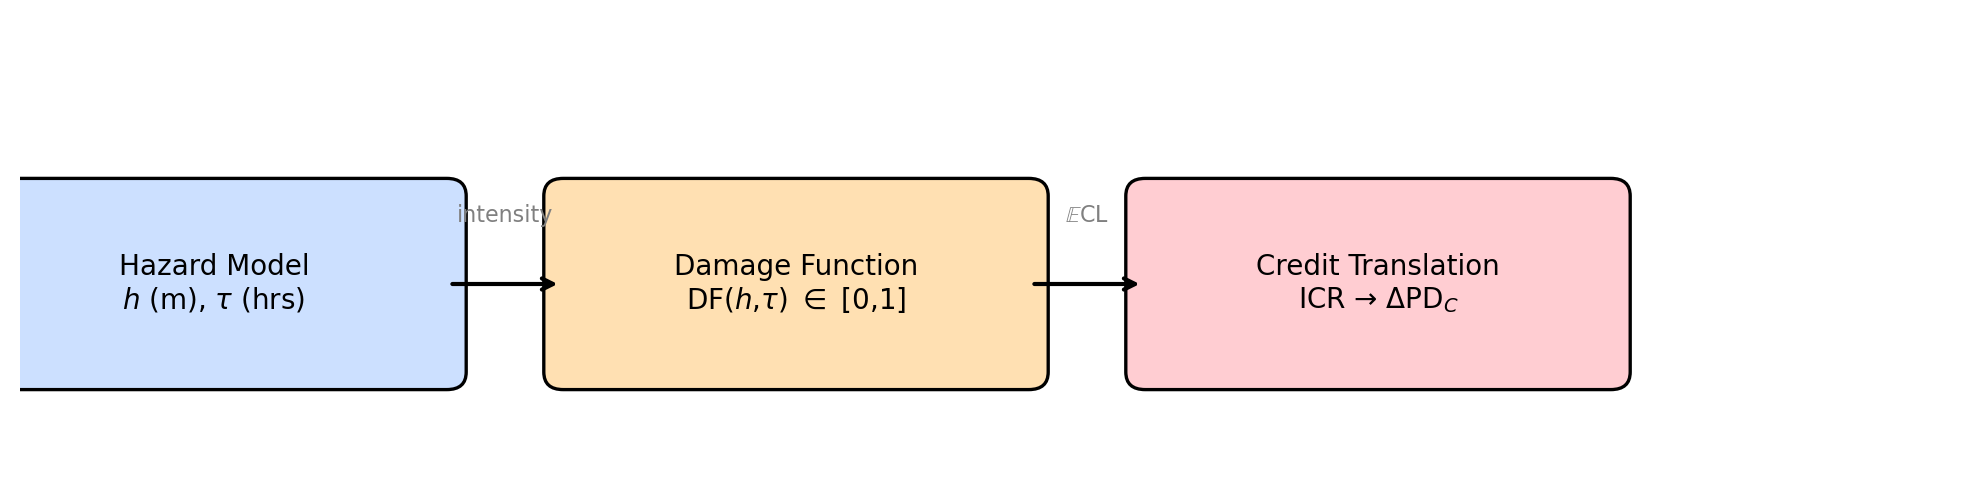
\includegraphics[width=0.85\textwidth]{Content/Images/pipeline_scheme.png}
\caption{Three-stage pipeline: hazard intensity is converted to a damage ratio via the parametric damage function (Sections~\ref{ssec: damage function}--\ref{ssec: sector}), then translated into a PD shift (Section~\ref{ssec: pd shift}).}
\label{fig: scheme}
\end{figure}

The \textit{hazard characterisation} stage provides the probability and intensity of physical hazards at each asset location. For floods, the key variables are water depth $h$ (metres) and inundation duration $\tau$ (hours), obtained from FEMA flood zone maps, hydrological models, or scenario-based projections. The \textit{damage estimation} stage converts hazard intensity into a damage ratio $\DF \in [0,1]$ via a parametric damage function. This is the primary methodological contribution of the paper: we extend the standard Richards function with duration dependence and calibrate it empirically (Sections~\ref{ssec: damage function}--\ref{ssec: sector}). The \textit{credit risk translation} stage converts expected monetary losses into a shift in probability of default $\Delta PD_C$, using the interest coverage ratio approach described in Section~\ref{ssec: pd shift}. This module is deliberately kept simple and replaceable --- more sophisticated models, including multi-ratio logistic regression~\cite{altman2007modelling, ohlson1980financial}, the Merton structural model~\cite{merton1974pricing}, or other approaches, can substitute for it without affecting the upstream damage estimation.

The data flow for a multi-location company proceeds as follows (Fig.~\ref{fig: dataflow}): asset locations are mapped to local hazard parameters, damage ratios are computed per facility, and losses are aggregated to the company level before credit translation.

\begin{figure}[ht]
\centering
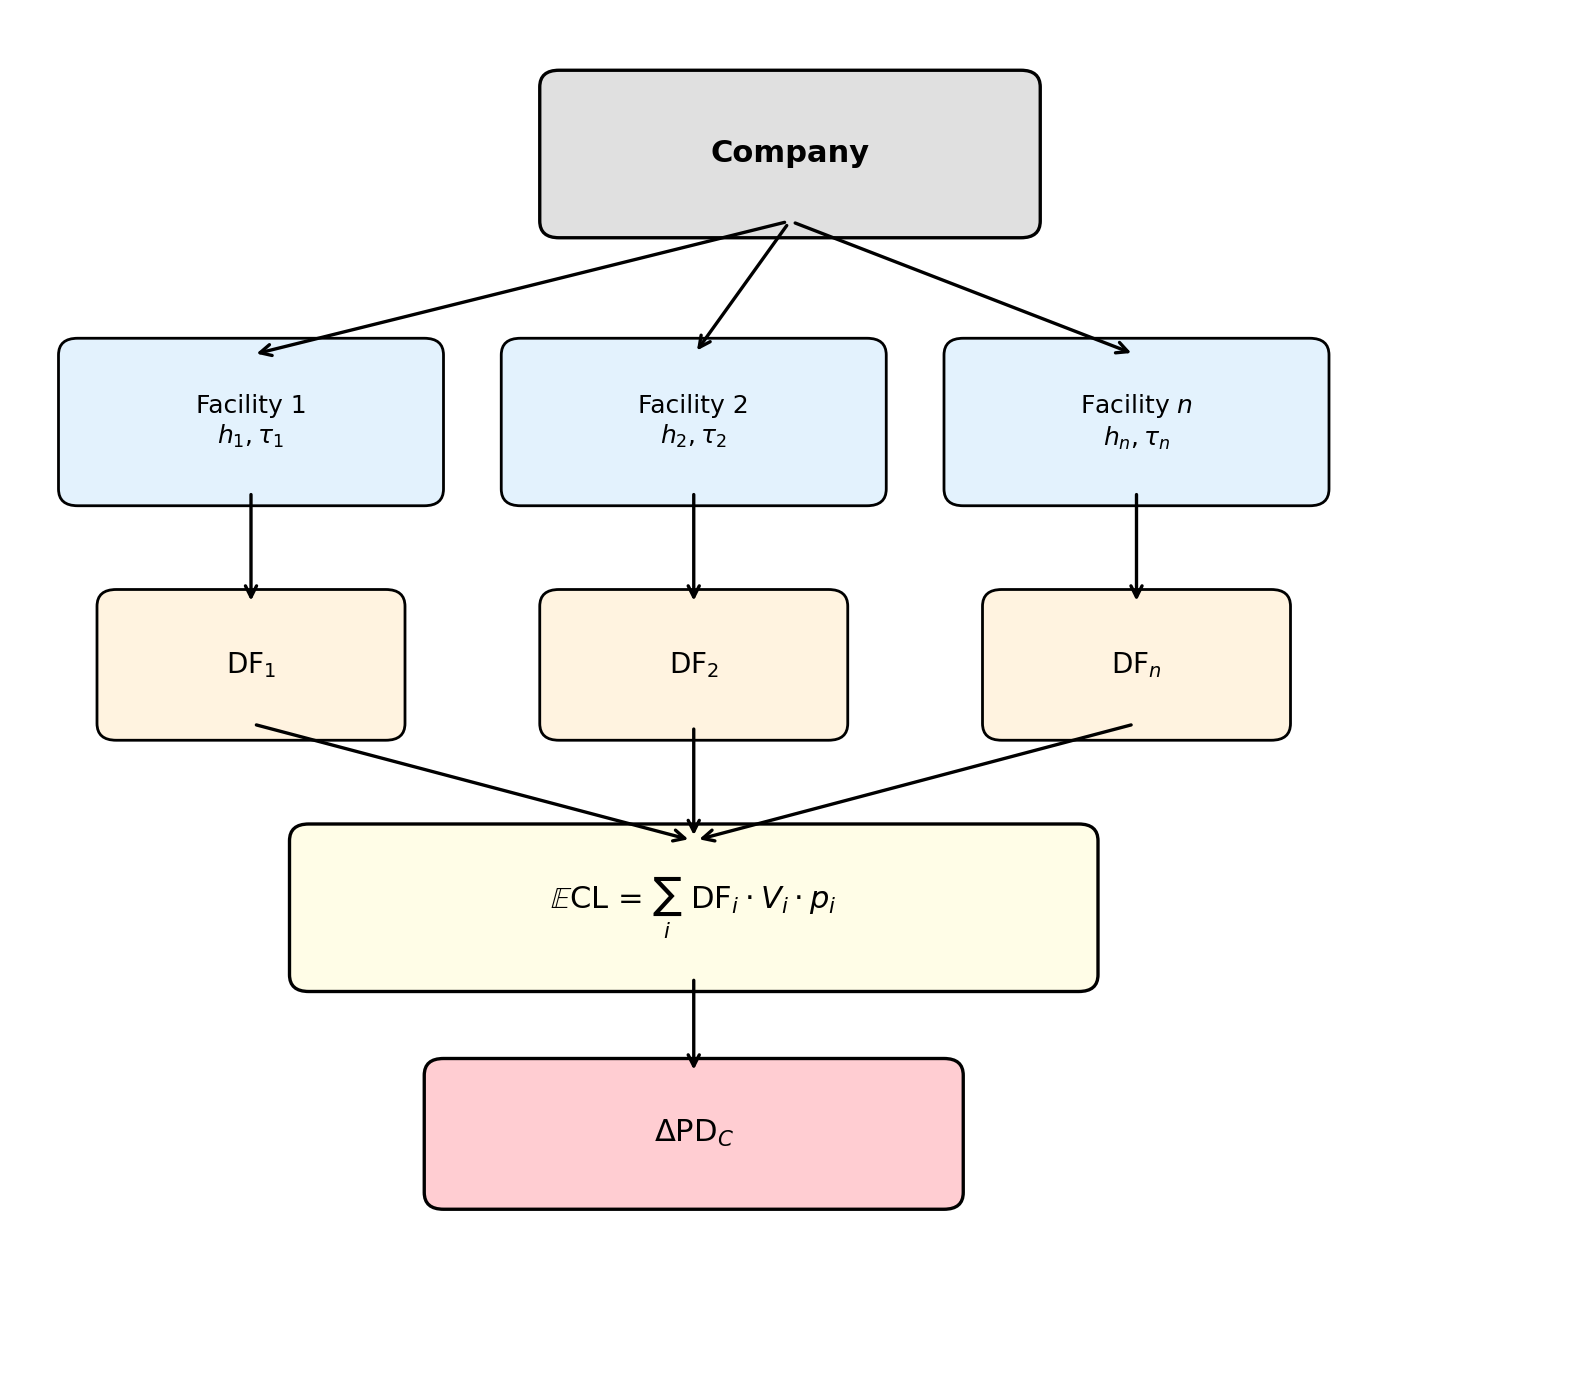
\includegraphics[width=0.55\textwidth]{Content/Images/dataflow_diagram.png}
\caption{Data flow for a multi-location company: each facility's hazard parameters are converted to a damage ratio, losses are aggregated by replacement value $V_i$ and event probability $p_i$, then translated into a PD shift.}
\label{fig: dataflow}
\end{figure}
